\section{Roboterkomponenten}
\textbf{Die Asimov’schen Gesetze}\newline
\begin{enumerate}
    \item Ein Roboter darf kein menschliches Wesen verletzen oder durch Untätigkeit zulassen, dass einem menschlichen Wesen Schaden zugefügt wird.
    \item Ein Roboter muss den ihm von einem Menschen gegebenen Befehlen gehorchen – es sei denn, ein solcher Befehl würde mit Regel eins kollidieren.
    \item Ein Roboter muss seine Existenz beschützen, solange dieser Schutz nicht mit Regel eins oder zwei kollidiert.
\end{enumerate}
\begin{minipage}{0.5\linewidth}
\end{minipage}
\begin{minipage}{0.5\linewidth}
    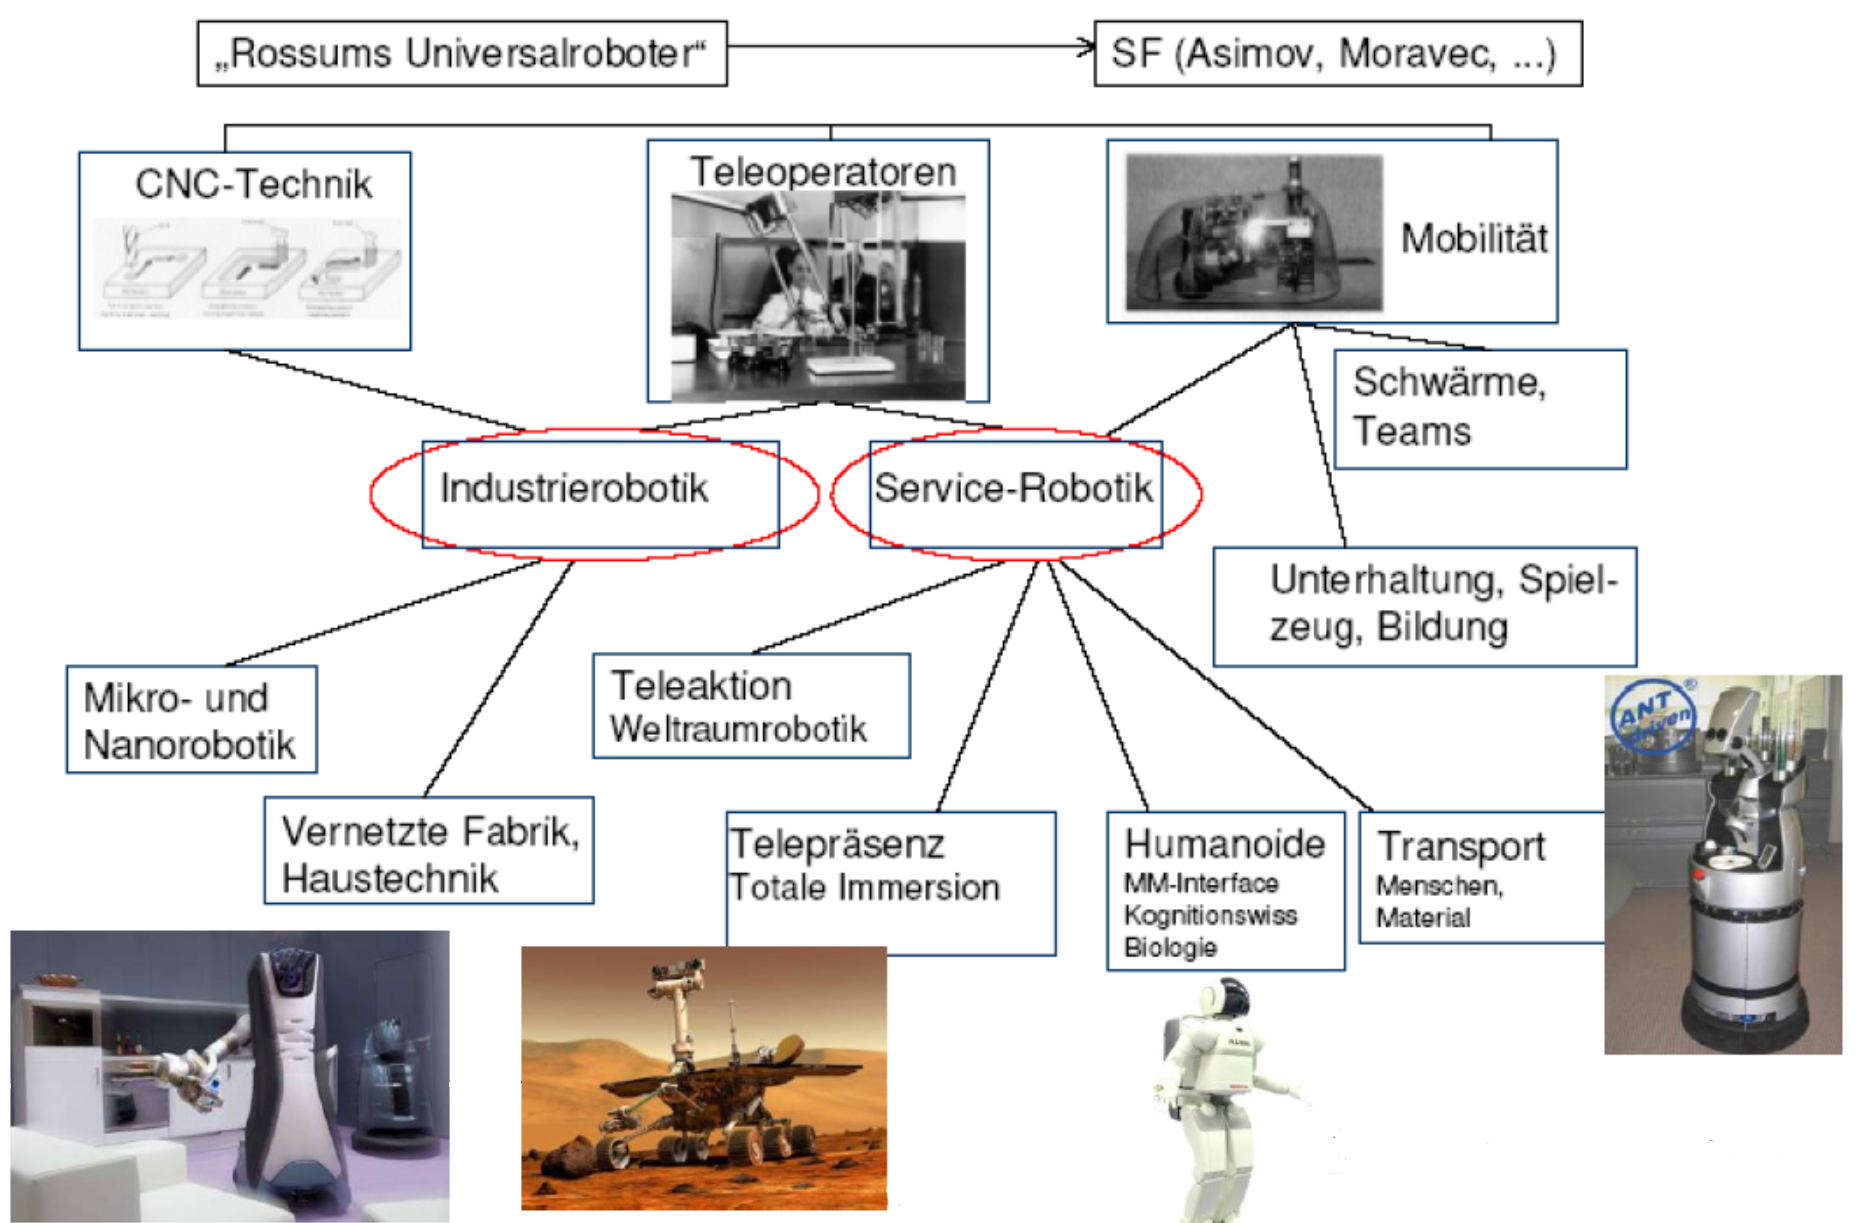
\includegraphics[width=\linewidth]{./bilder/RoboAnwendung}
\end{minipage}
\begin{minipage}{0.5\linewidth}
    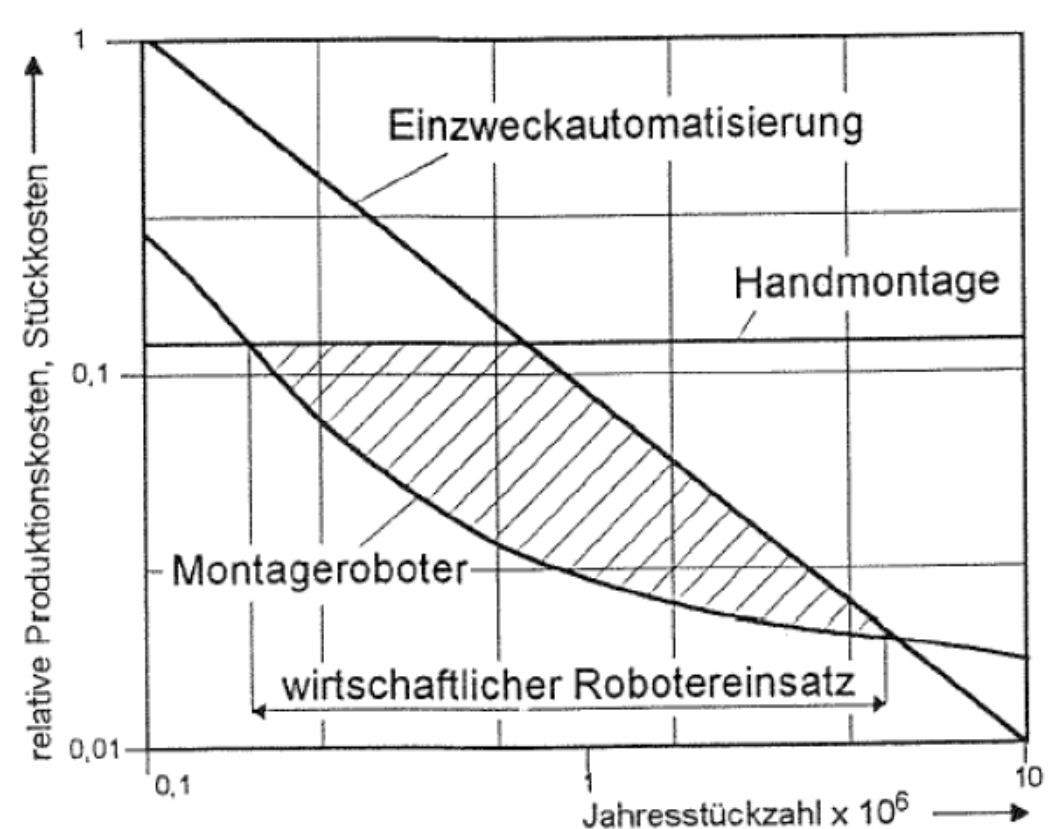
\includegraphics[width=0.9\linewidth]{./bilder/RoboWirtsch}
\end{minipage}
\subsubsection{Definition Roboter}
\begin{minipage}[t]{0.48\linewidth}
    \subsubsection{industrial robot}
    An automatically controlled, reprogrammable, multipurpose manipulator programmable in three or more axes, which may be either fixed in place or mobile for use in industrial automation applications.
\end{minipage}\hspace{0.04\linewidth}
\begin{minipage}[t]{0.48\linewidth}
    \subsubsection{service robot}
    A robot which operates semi-or fully autonomously to perform services useful to the well-being of humans and equipment, excluding manufacturing operations.
\end{minipage}
\subsection{Wachstum}
Die Haupttreiber für Autmation und somit für den Roboterwachstum sind:
\begin{itemize}
    \item Energieeffizienz und neue Materialien wie Kohleverbundstoffe, erfordern neu Produktionen.
    \item Globale Wettbewerbsfähigkeit erfordert höhere Produktivität und Qualität.
    \item Wachsende Verbrauchermärkte erfordern die Erweiterung von Produktionskapazitäten.
    \item Kürzere Produktlebenszyklen sowie steigende Produktvielfalt erfordern flexible Automation
    \item Roboter verbessern die Arbeitsplatzqualität bei gefährlichen, anstrengenden und schmutzigen Arbeiten, die für Menschen zu gefährlich oder undurchführbar sind.
\end{itemize}
\begin{minipage}{0.5\linewidth}
    \subsection{Genauigkeit}
    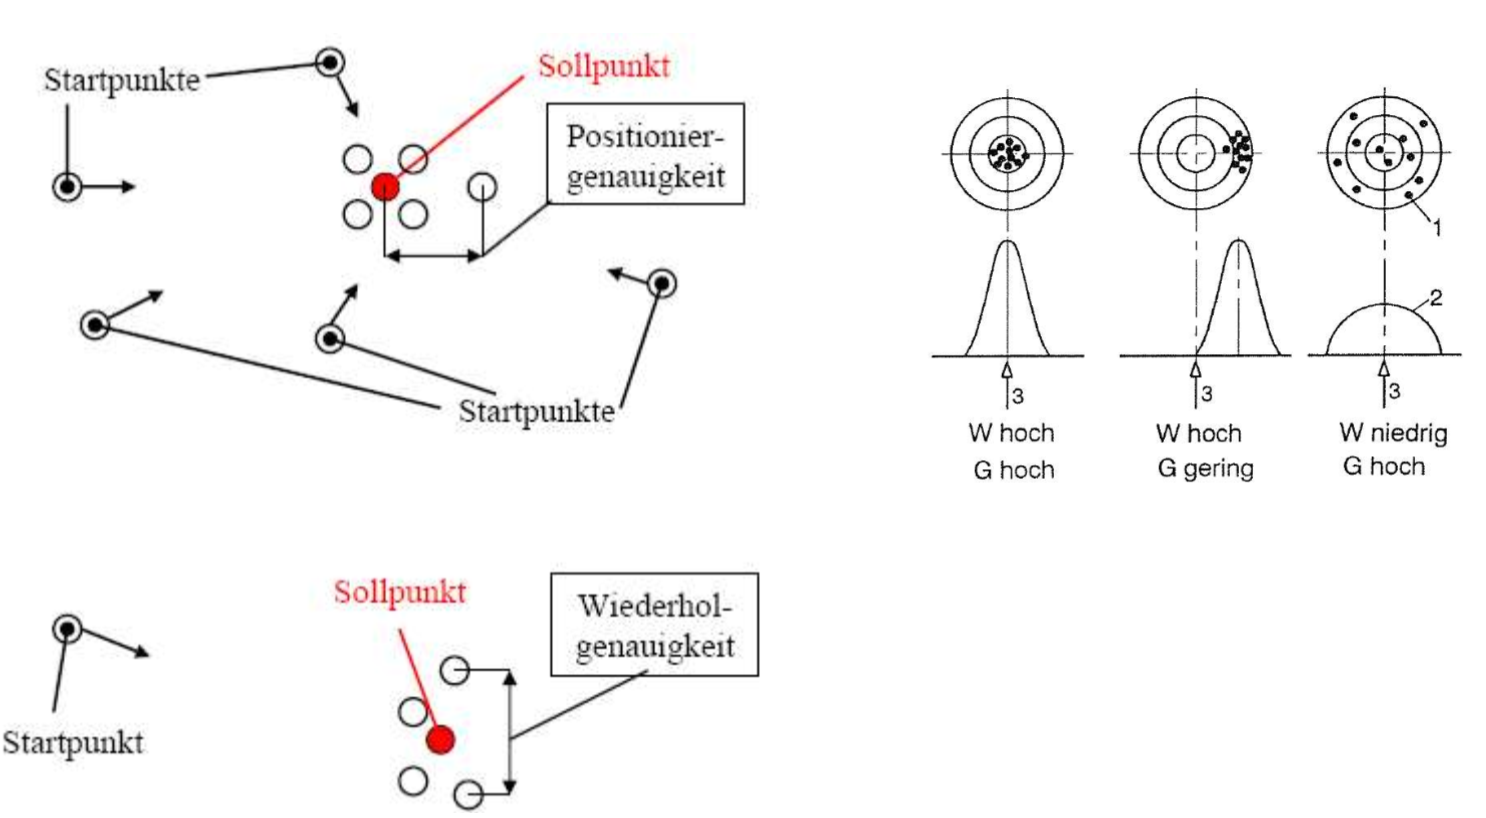
\includegraphics[width=\linewidth]{./bilder/genauigkeit}
\end{minipage}
    \begin{minipage}{0.5\linewidth}
    \subsection{Anlage}
    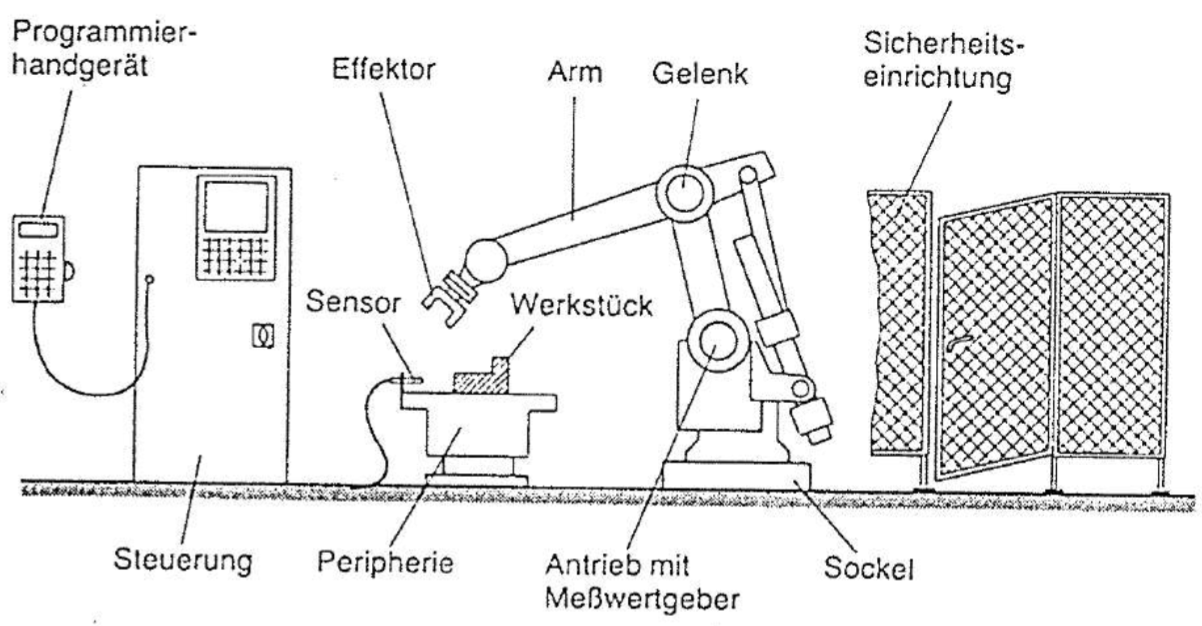
\includegraphics[width=\linewidth]{./bilder/anlage}
\end{minipage}
\clearpage
\subsection{Charakterisierung}
\vspace{-0.5cm}
\begin{multicols}{2}
    \small
\begin{itemize}
    \item Mobility -or also number of degrees of freedom (dof)
    \begin{itemize}
        \item defines how the robot can translate and rotate objects in space
        \item m: mobility needed for the applicat
        \item n: mobility of the robot
        \item sometimes we choose n>m (easier to integrate, or to avoid obstacles, …)
    \end{itemize}
    \item Handling capacity
    \begin{itemize}
        \item capacitygives the mass that can be handled by the robot (including the mass of the gripper or the tool)
    \end{itemize}
    \item Workspace
    \begin{itemize}
        \item defines the volume that can be reached by the wrist of the robot. The shape of the workspace is often important for a given application.
    \end{itemize}
    \item Maximal speed and acceleration
    \begin{itemize}
        \item defines how fast the robot can move
        \item speed and acceleration are often given for the individual axes of the robot
        \item acceleration capability is especially important for small displacements, for which the maximal speed cannot be reached.
        \item in some cases, a cycle time is given, which is the time required for one typical pick and place motion
    \end{itemize}
    \item Environment
    \begin{itemize}
        \item EnvironmentTo select a robot for a given application it is important to specify the environment in which it is going to be used. For example, the robot can be affected by the environment but it can also pollute its environment. Care has to be given when selecting a robot for following environments: clean rooms, food industry and explosive environments
    \end{itemize}
    \item Accuracy (Positioniergenauigkeit)
    \begin{itemize}
        \item is usually not given, because it is low. To obtain a good accuracy, a calibration of the robot is necessary.
    \end{itemize}
    \item Repeatability (Wiederholgenauigkeit)
    \begin{itemize}
        \item it is usually the measure of precision given by the robot manufacturer. It gives the capability of the robot to come back to the same position after it has been moved.
    \end{itemize}
    \item Resolution
    \begin{itemize}
        \item smallest mechanical step the machine can make during point-to-point motion
    \end{itemize}
\end{itemize}
\end{multicols}
\enlargethispage{1cm}
\begin{minipage}{0.5\linewidth}
\subsection{Anforderungen}
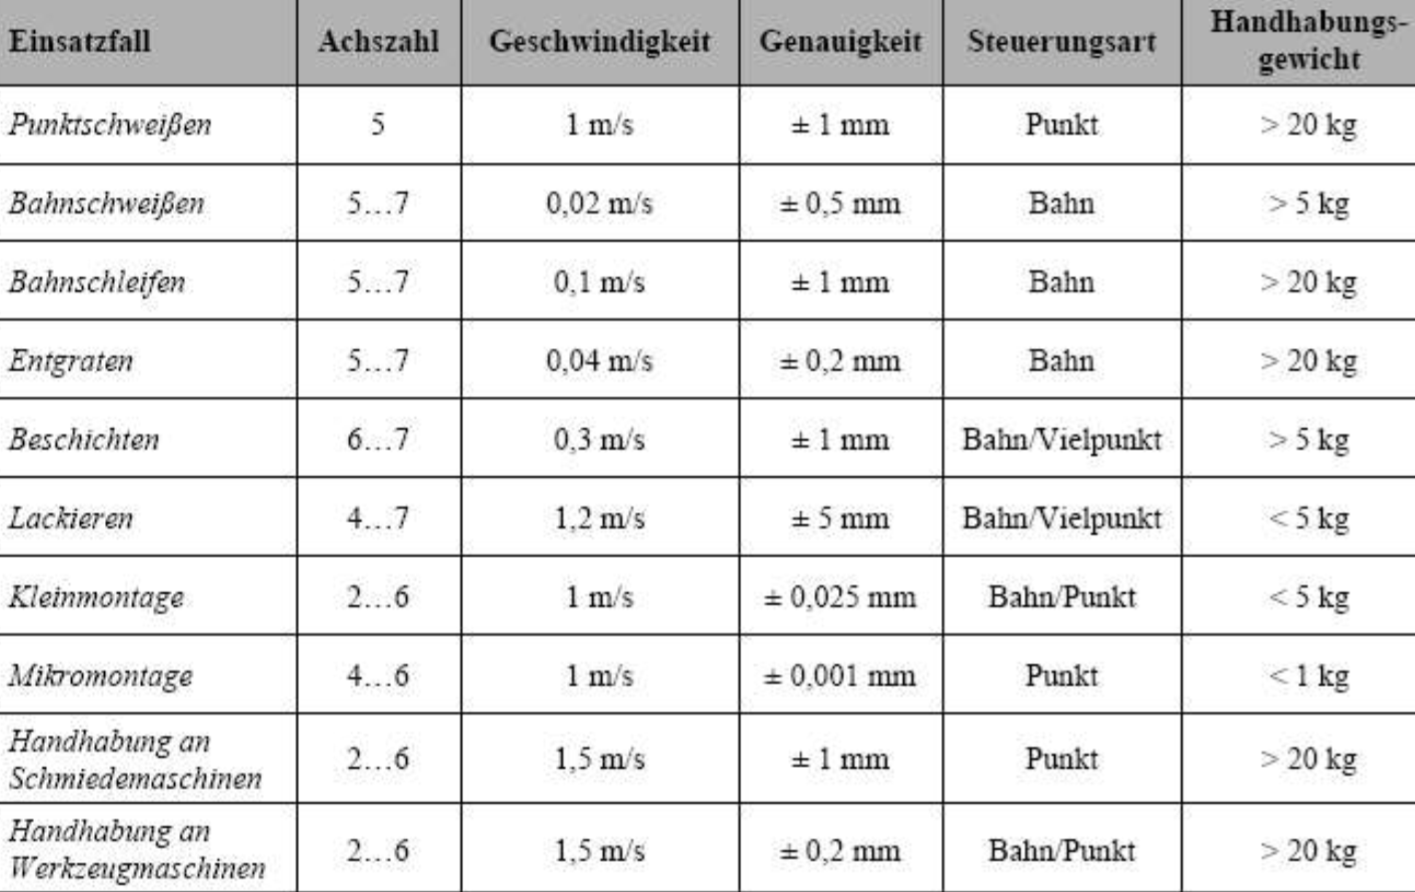
\includegraphics[width=\linewidth]{./bilder/anforderung}
\end{minipage}
\begin{minipage}{0.5\linewidth}
{\small 
\begin{tabular}{lcp{5.3cm}}
	\textbf{Art}& \textbf{FG}&\textbf{Grund}\\
	Punktschweissen& 5& Werkzeug rotationssymetrisch\\
	&(6)&(+1 für Kollisionsvermeidung)\\
	Bahnschweissen&6&Schweissen im Raum, Kollisionsvermeidung\\
	Laserschneiden&5&Werkzeug rotationssymetrisch\\
	Palettieren&4&Paletten in einer Ebene, 1 Rotationsachse für Orientierung\\
	Platinen bestücken&4&Platzieren 2, Höhe 1, Orientieren 1\\
	&&\\
\end{tabular}
}
\end{minipage}

\begin{minipage}{0.5\linewidth}
    \subsection{Komponent}
    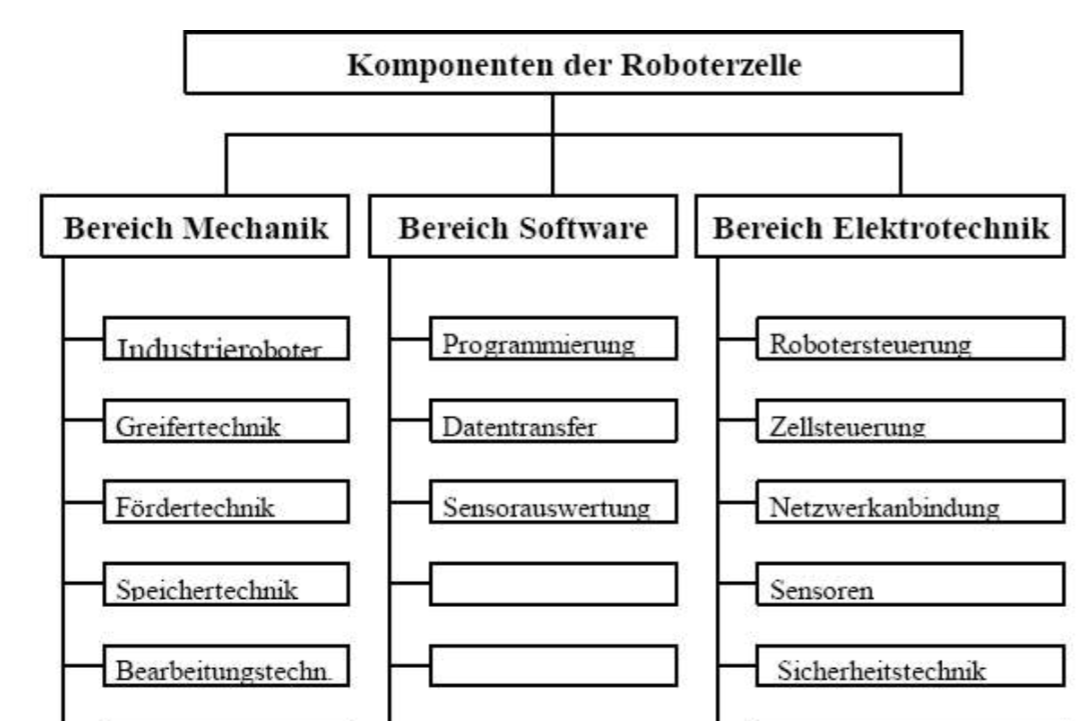
\includegraphics[width=\linewidth]{./bilder/komponent}
    
\end{minipage}
\begin{minipage}{0.5\linewidth}
    \vspace{-0.5cm}
    \subsection{Freiheitsgrade \robo{43}{2.1.9}}
    Anzahl der möglichen unabhängigen Bewegungen eines starren Körpers gegenüber einem Bezugskoordinatensystem. Max. nötig 6 (3 Translationen, 3 Rotationen). Ein Roboter kann mehr als 6 FG haben um Kollisionen zu vermeiden. Die Schliessbewegung des Greifers zählt nicht als FG.
    
    \subsection{Singularität \robo{58}{3.2.1}}
    Armstellung, bei der sich der FG der Kinematik reduziert.
    \subsubsection{Singuläre Konfiguraion}
    Die Drehung einer Achse kann durch die Gegendrehung einer anderen Achse kompensiert werden.
    Ein FG geht verloren, da für eine Drehachse zwei Gelenke verwendet werden.
    \subsubsection{Grenzsingularität}
    Der Roboter ist ganz ausgrstreckt oder an der Position am rande des Arbeitsbereichs. Er kann sich nicht mehr in alle Richtungen bewegen
\end{minipage}

\clearpage
\section{Kinematik}
Eine kinematische Kette besteht aus Armen/Körper verbunden mit Gelenken so das sie die rotatorische und translatorische bewegungen ausführen kann.
\subsection{Aufbau}
\begin{minipage}{0.5\linewidth}
\subsubsection{Seriell}
\begin{itemize}
    \item Das erste Armglied ist fest mit dem Boden/Sockel verbunden.
    \item Am letzten Armglied ist ein Effektor befestigt.
    \item An jedem Armgield befindet sich nur ein Gelenk, welches das nächste Armglied verbindet.  
\end{itemize}
\end{minipage}
\begin{minipage}{0.5\linewidth}
\subsubsection{Parallel}
\begin{itemize}
    \item mindestens einen geschlossenen kinematische Kette.
    \item entsteht, wenn ein Armteil auf zwei verschiedenen Wegen mit dem Sockel vebrunden ist.
\end{itemize}
\end{minipage}
	\subsection{Darstellung kinematischer Gelenke \robo{46}{2.2.1}}
    \enlargethispage{1cm}
\begin{minipage}{10cm}
	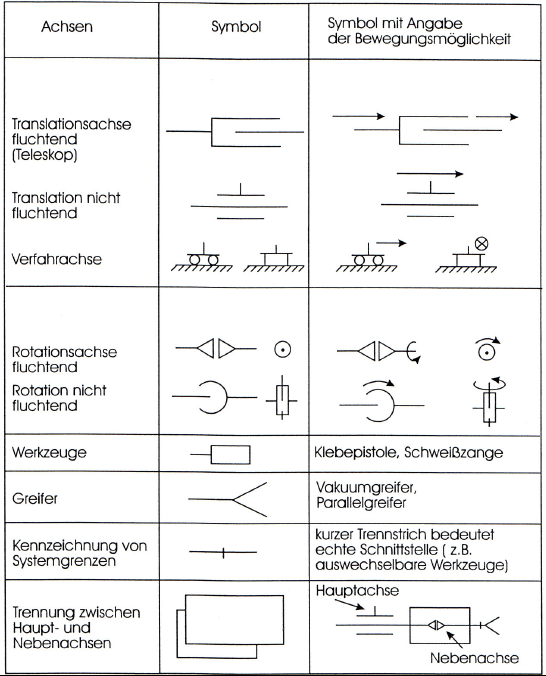
\includegraphics[width=10cm]{./bilder/symbole}
\end{minipage}
\begin{minipage}{5.1cm}
	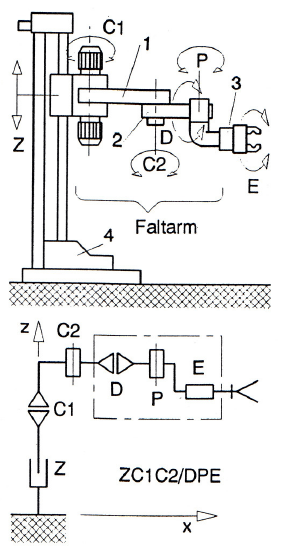
\includegraphics[width=5cm]{./bilder/symbole-bsp}
\end{minipage}
\begin{minipage}{0.2\linewidth}
    \textbf{Weitere Darstellungen:}\newline
    \robos{46}\newline
    \robos{47}\newline
    \robos{51}\newline
    \robos{52}\newline
    \robos{54}\newline
    \robos{60}
\end{minipage}


\begin{minipage}{0.5\linewidth}
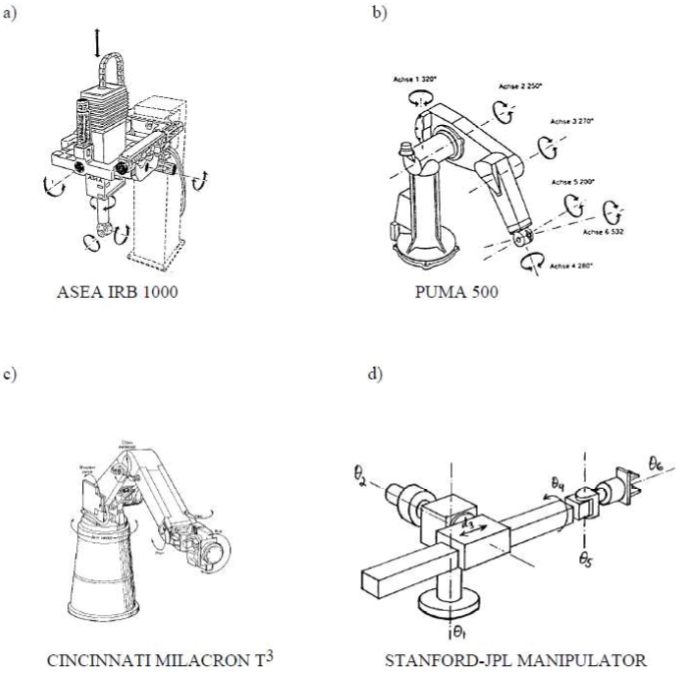
\includegraphics[width=0.8\linewidth]{./bilder/KinAuf}
\end{minipage}
\begin{minipage}{0.5\linewidth}
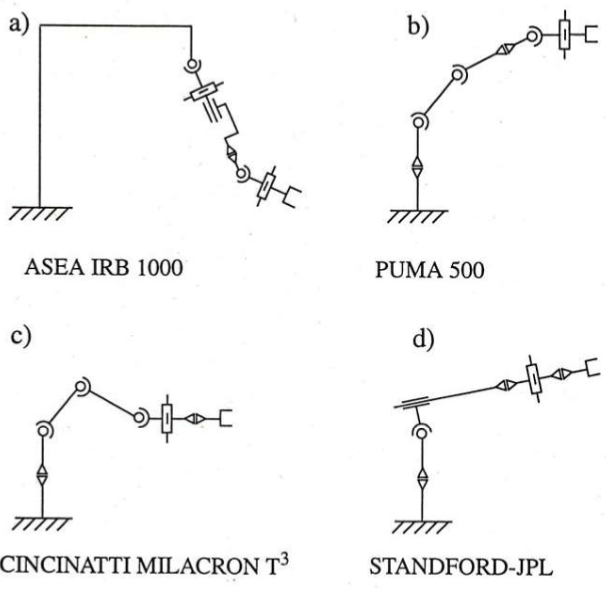
\includegraphics[width=0.8\linewidth]{./bilder/KinAufL}
\end{minipage}
\clearpage
\begin{minipage}{0.5\linewidth}
    \subsection*{Vergleich}
    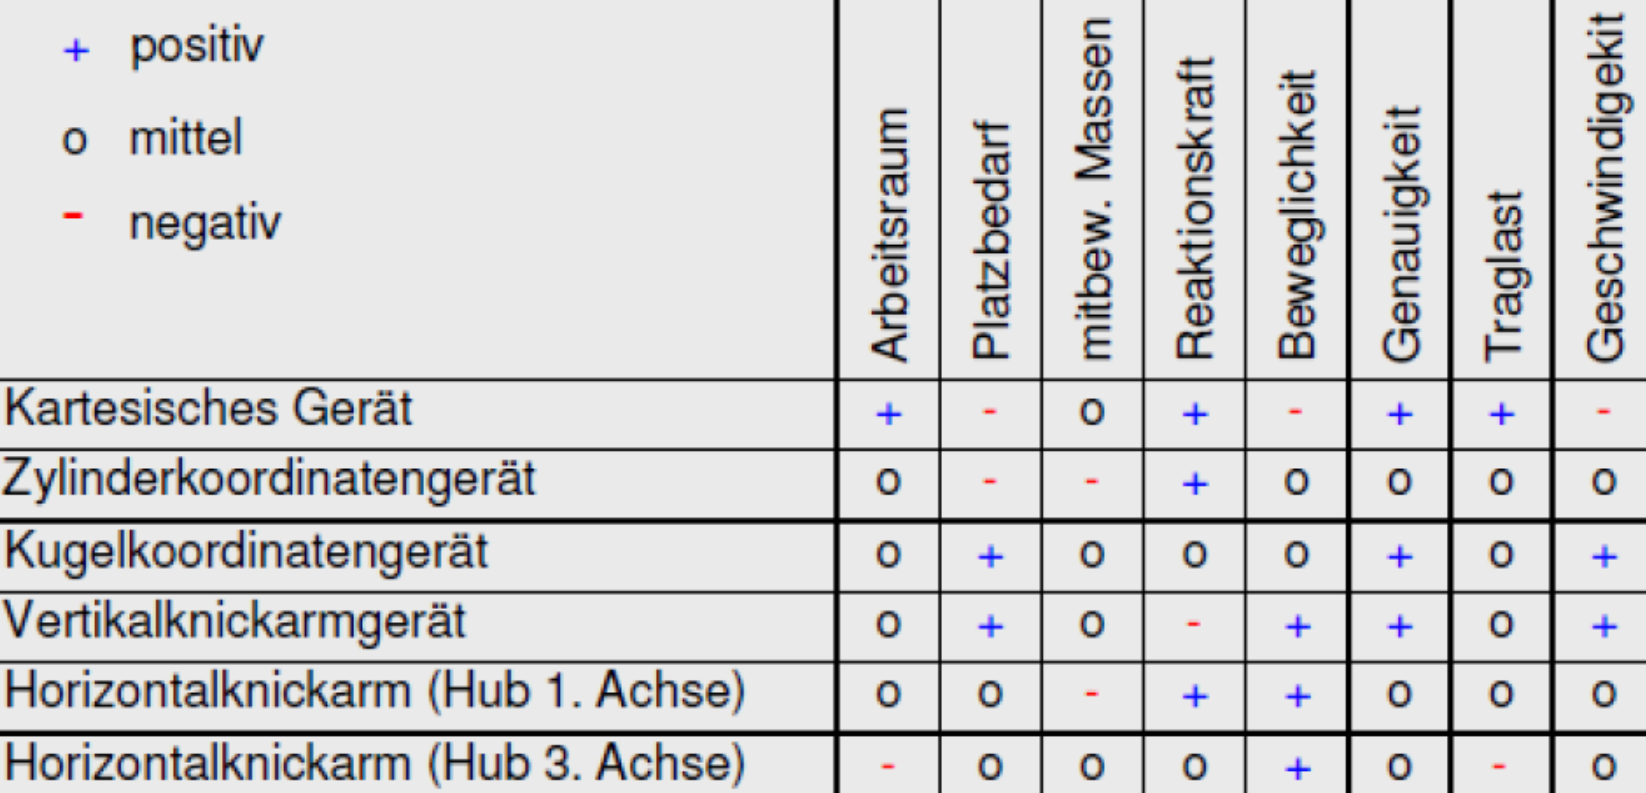
\includegraphics[width=\linewidth]{./bilder/RoboVergleich}
%\end{minipage}   
%\begin{minipage}{0.4\linewidth}
    \subsubsection{Kartesischer Roboter}
    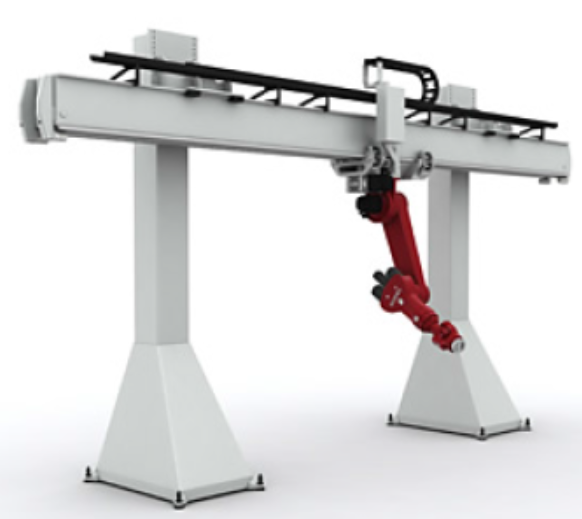
\includegraphics[height=3cm]{./bilder/PortalRobo}
    
    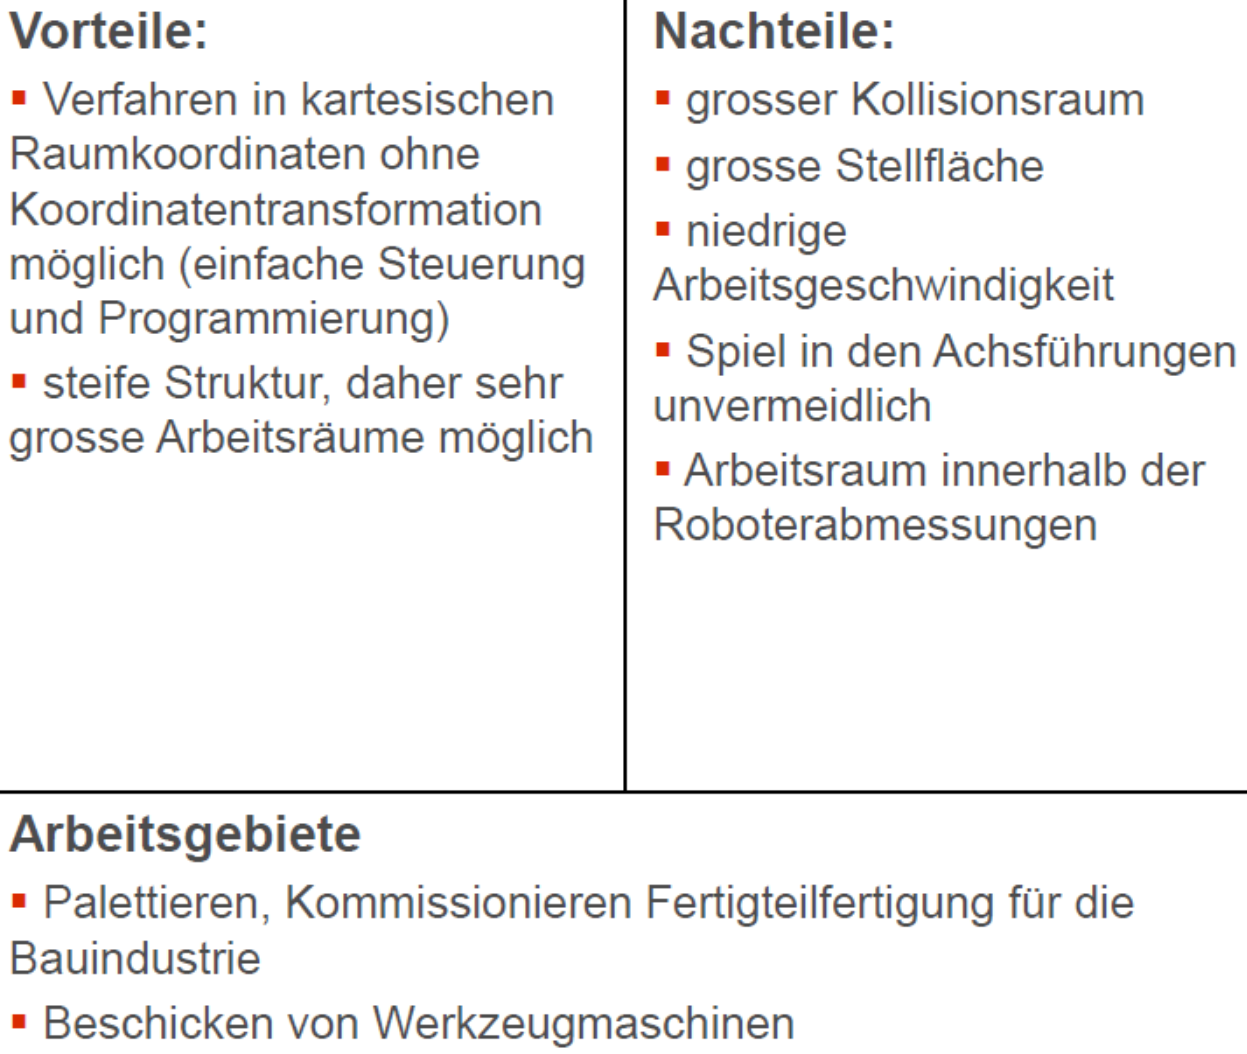
\includegraphics[width=\linewidth]{./bilder/kartRobo}
\end{minipage}
\begin{minipage}{0.5\linewidth}
    \subsection{Robotertypen}
    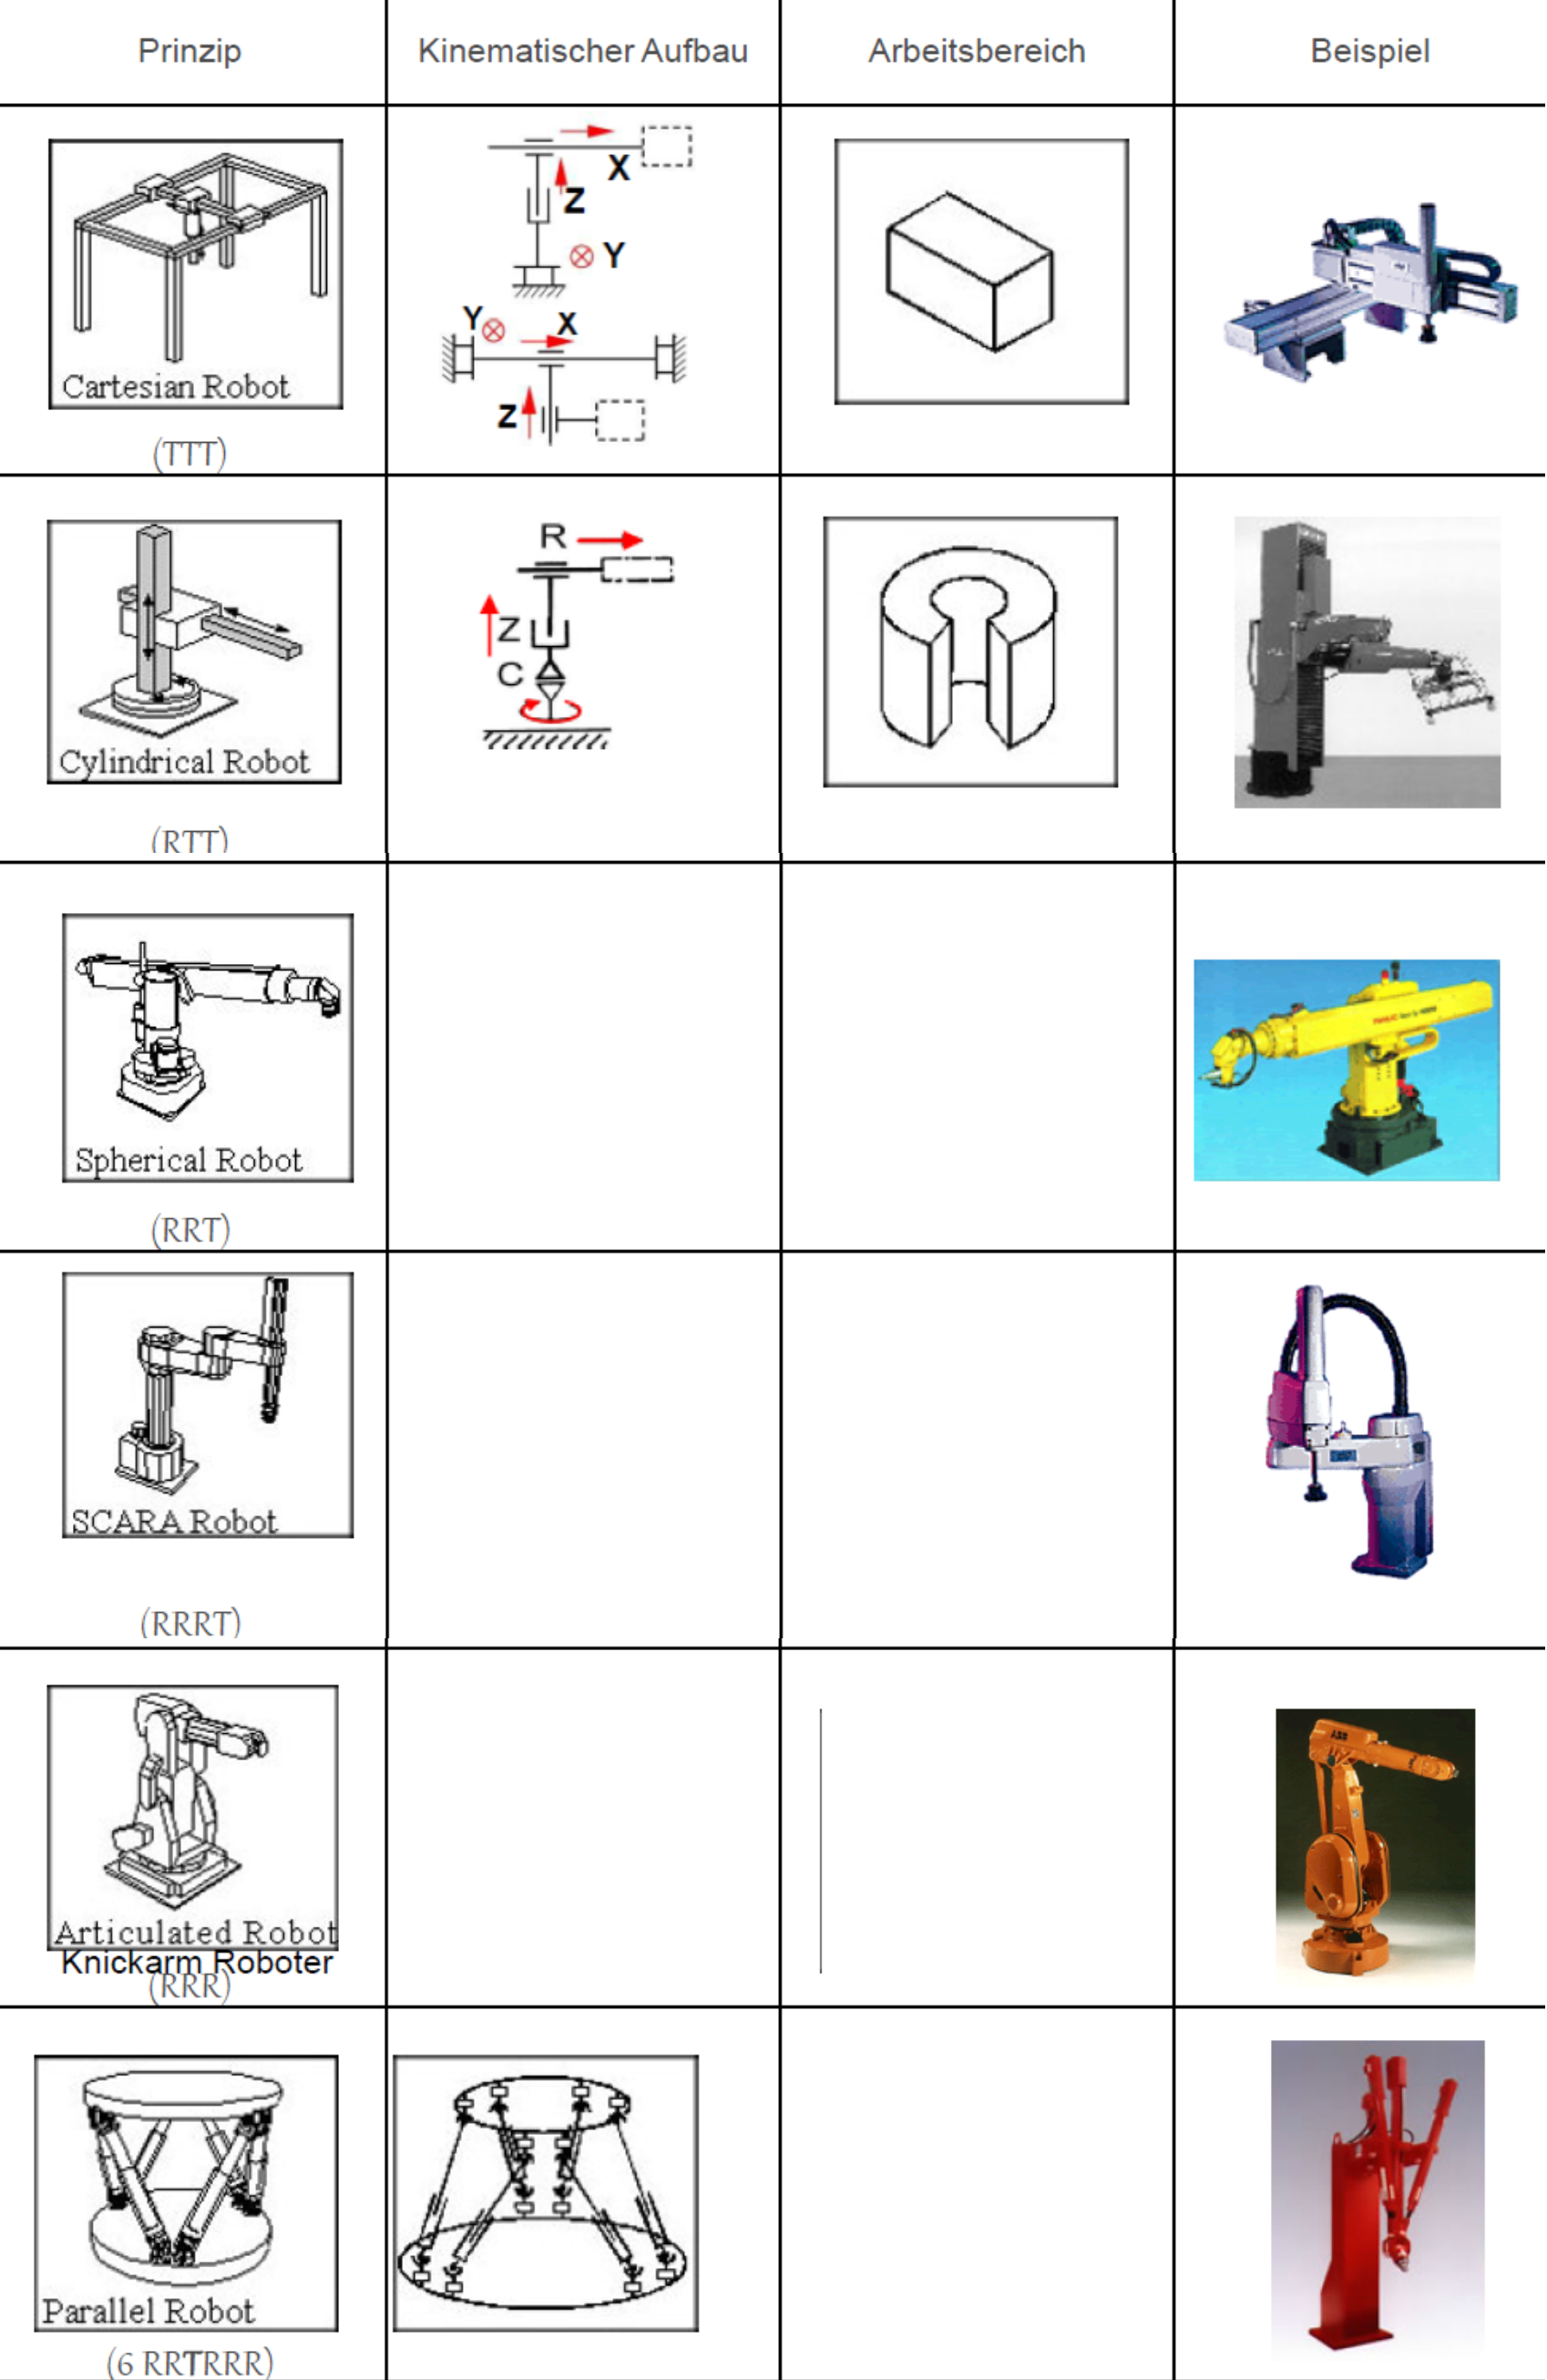
\includegraphics[width=\linewidth]{./bilder/RoboTypen}
\end{minipage}

\begin{minipage}{0.33\linewidth}
    \subsubsection{SCARA Roboter}
    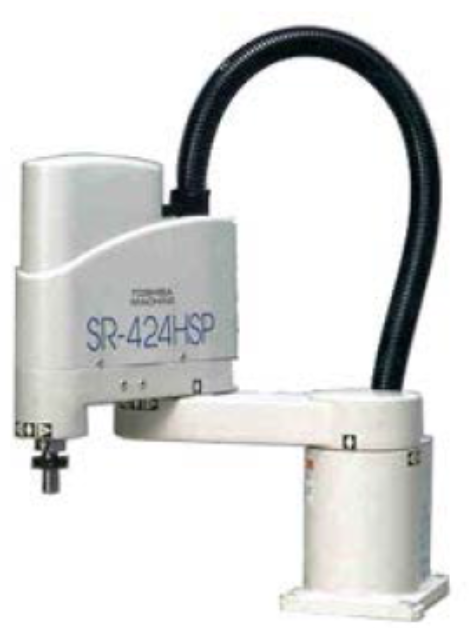
\includegraphics[height=3cm]{./bilder/ScaraRoboBsp}
    
    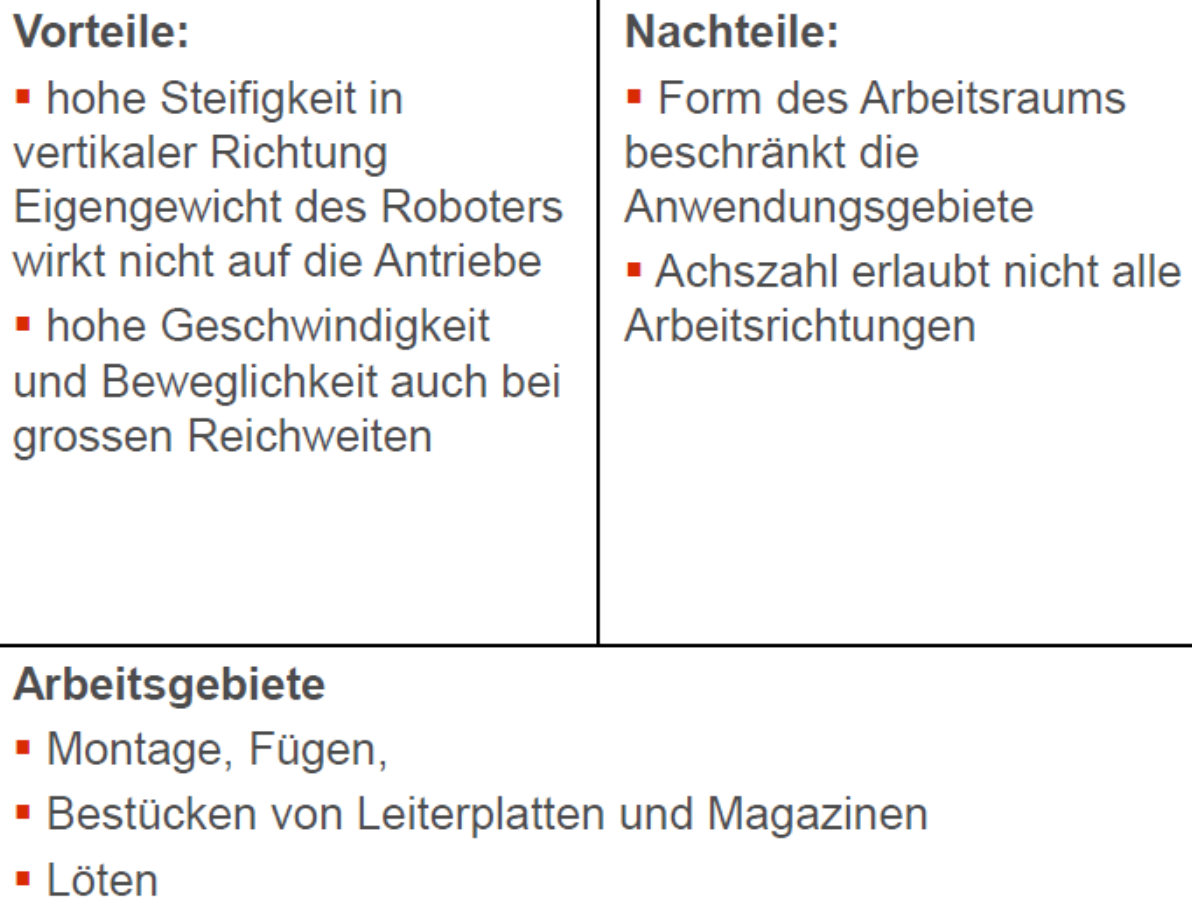
\includegraphics[width=\linewidth]{./bilder/ScaraRobo}
\end{minipage}
\begin{minipage}{0.33\linewidth}
    \subsubsection{Vertikal-Knickarmroboter}
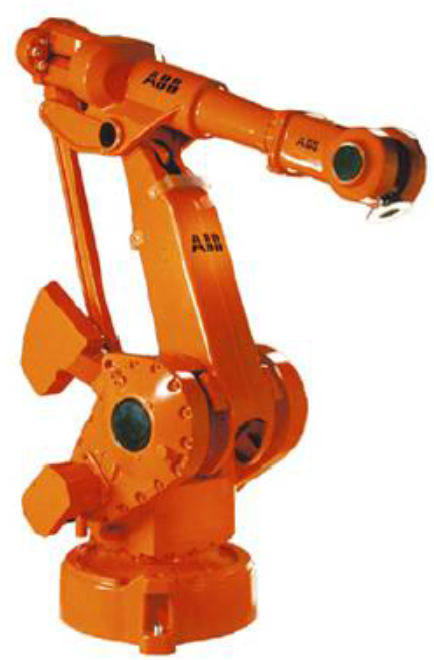
\includegraphics[height=3cm]{./bilder/KnickarmRoboBsp}

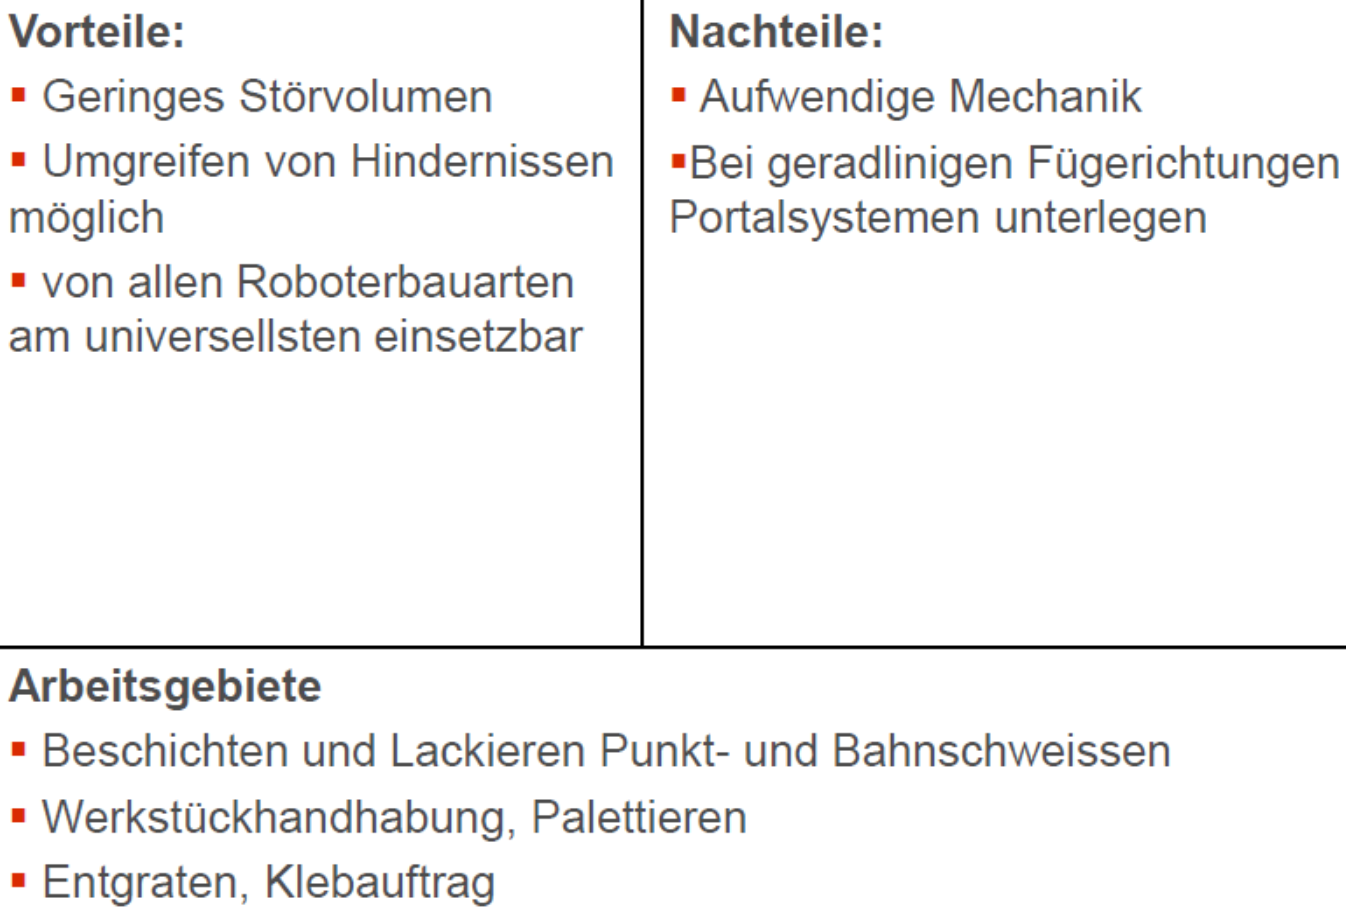
\includegraphics[width=\linewidth]{./bilder/KnickarmRobo}
\end{minipage}
\begin{minipage}{0.33\linewidth}
    \subsubsection{Parallelroboter}
    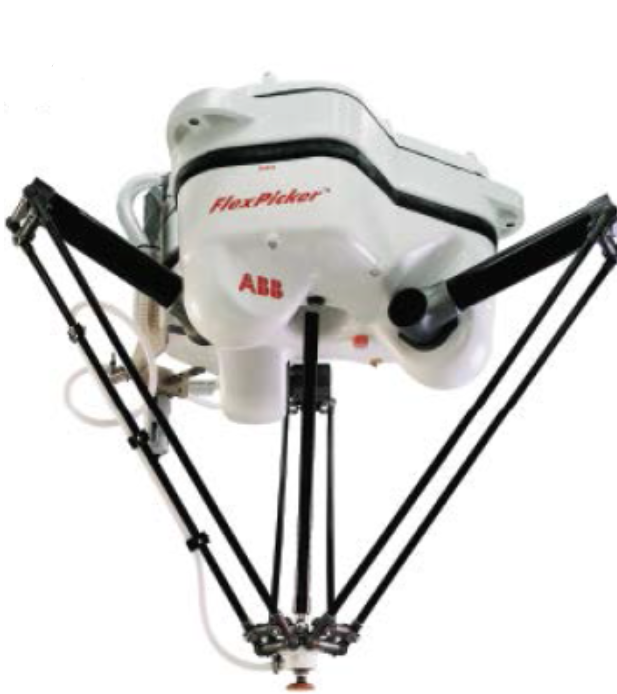
\includegraphics[height=3cm]{./bilder/ParallelRoboBsp}
    
    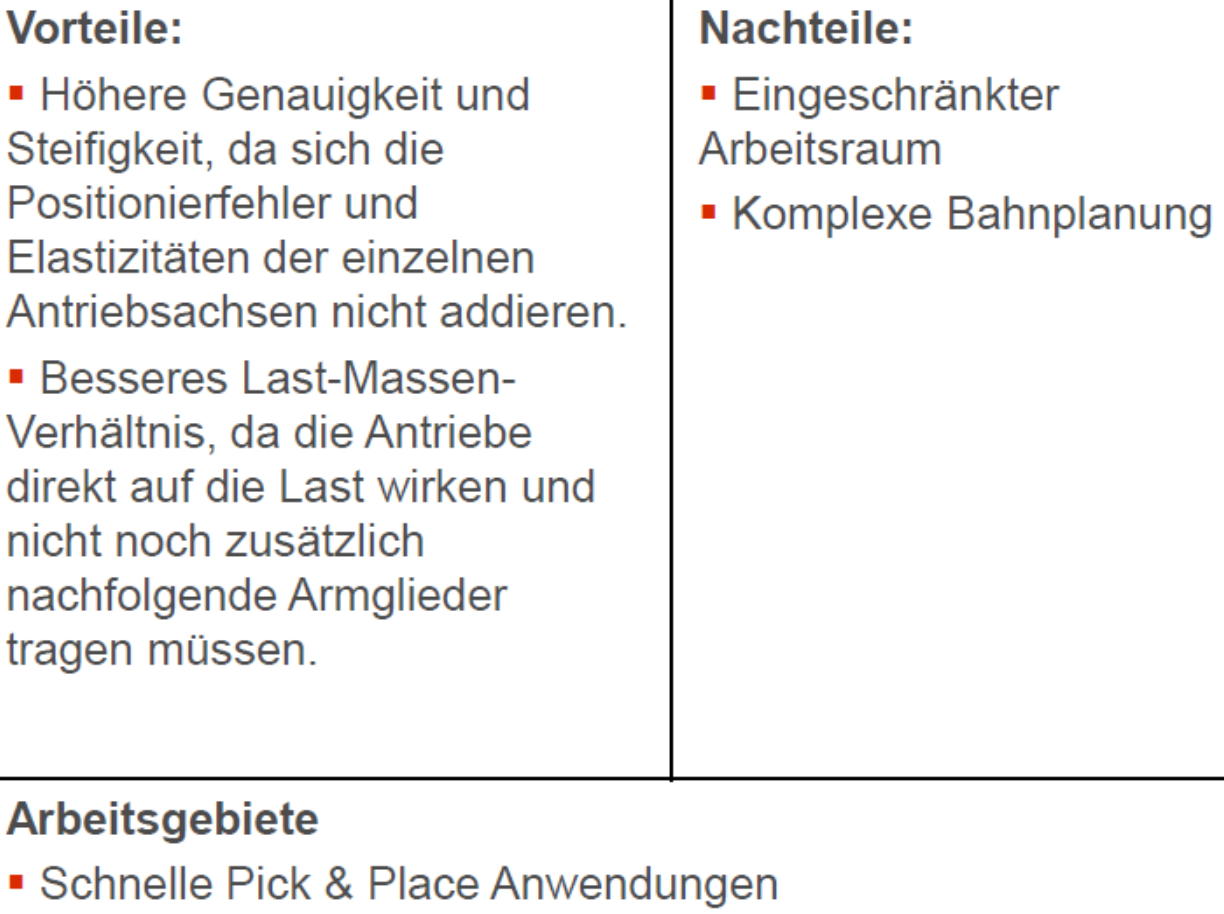
\includegraphics[width=\linewidth]{./bilder/ParallelRobo}
\end{minipage}

